
% ----------------------------------------------------------
% Desenvolvimento
% ----------------------------------------------------------
\chapter{Avaliação e Resultados}\label{sec:testes-resultados}
% ----------------------------------------------------------

% ----------------------------------------------------------
\section{Testes e Resultados}\label{sec:testes-resultados}
% ----------------------------------------------------------

Após o desenvolvimento de todos os módulos, a aplicação estava pronta para testes. Como os testes de erros e \textit{bugs} foram realizados após cada módulo, com sucesso, nessa parte somente foi testado a capacidade e geração dos dados.

O software pm2 foi configurado para executar o aplicativo, monitorar erros, fechamentos inexperados, entre outros, e os testes foram iniciados na seguinte sequência:

\begin{alineas}
	\item \textbf{Primeiro teste}: descoberta de cada \textit{beacon} MPact individualmente, a diferentes distâncias (\autoref{fig:peacon1});
	\item \textbf{Segundo teste}: descoberta de mais de um \textit{beacon} MPact simultaneamente, alternando um, dois e três a diferentes distâncias (\autoref{fig:peacon2});
	\item \textbf{Terceiro teste}: \textit{beacons} MPact em movimento, a diferentes distâncias;
	\item \textbf{Quarto teste}: mistura de \textit{beacons} MPact com iPad e Moto Maxx, diferentes quantidades e distâncias (\autoref{fig:peacon3} e \autoref{fig:peacon4});
	\item \textbf{Quinto teste}: diferentes localizações dos \textit{beacons} MPact, no bolso da calça com o usuário parado e em movimento.
\end{alineas}

\begin{figure}[htb]
	\centering
 	\begin{minipage}{0.45\textwidth}
		\centering
		\caption{\label{fig:peacon1}Identificação de um único \textit{beacon}}
		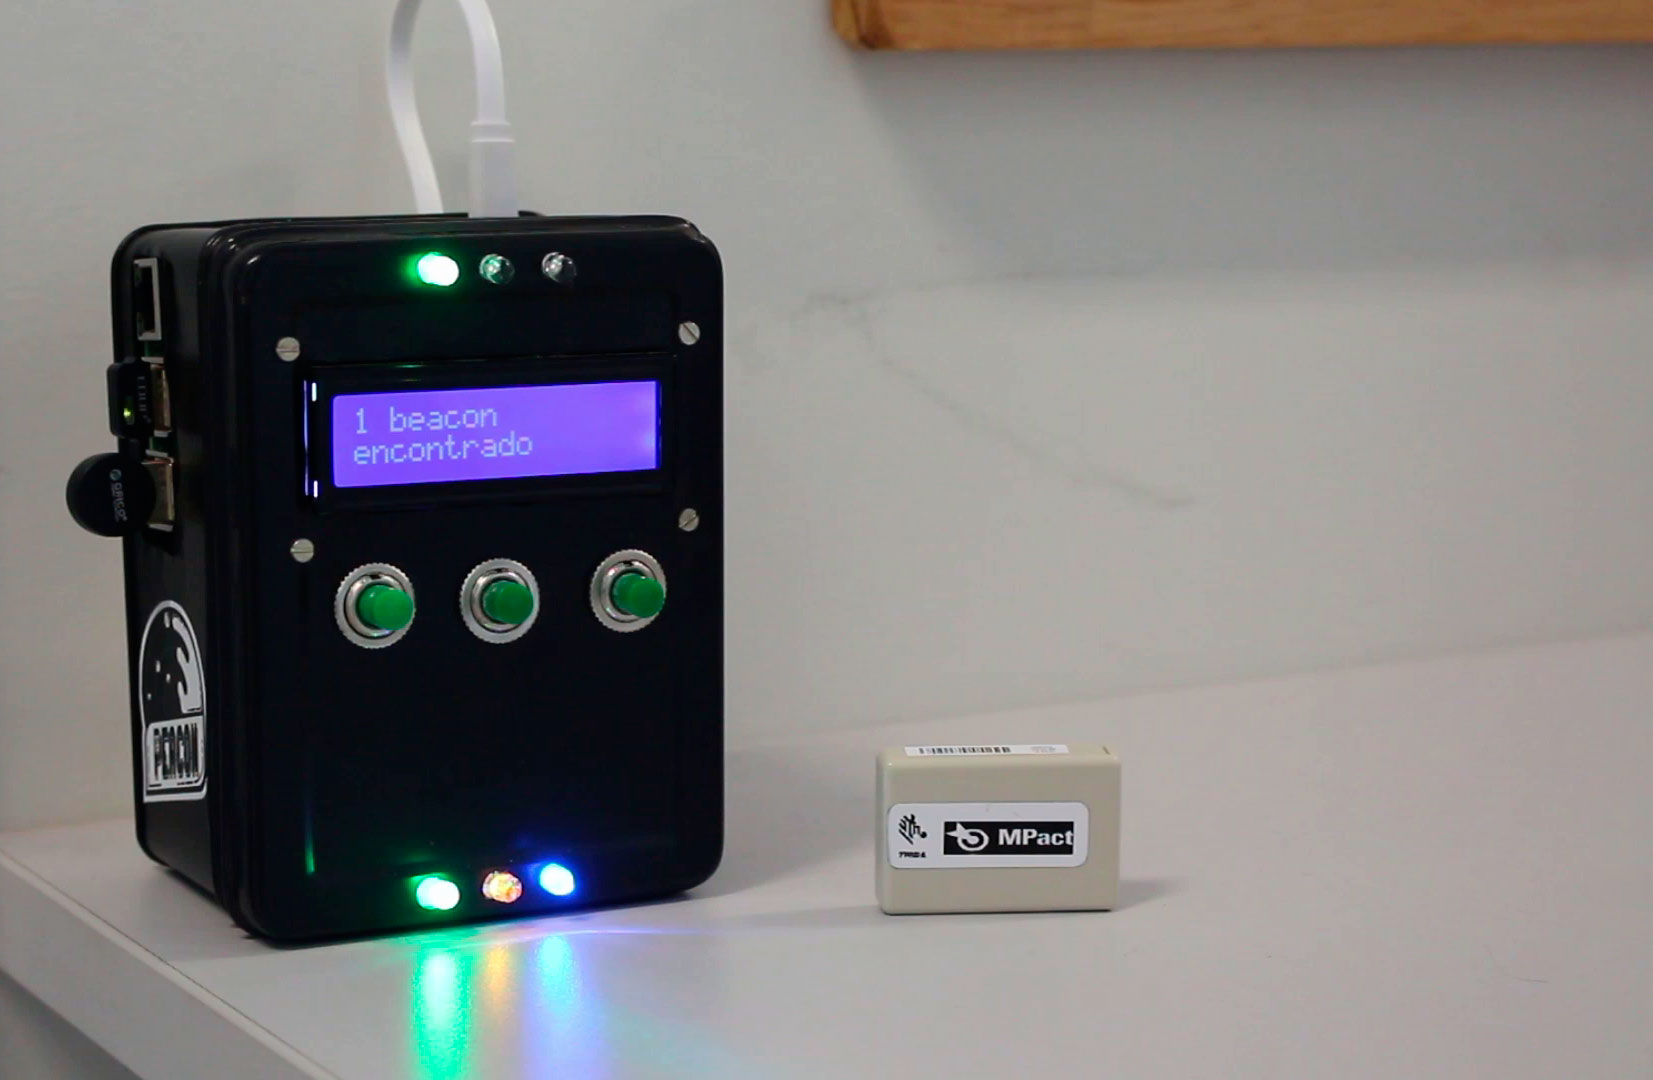
\includegraphics[width=1\textwidth]{img/peacon1.jpg}
		\legend{Fonte: elaborado pelo autor}
	\end{minipage}
	\hfill
	\begin{minipage}{0.45\textwidth}
		\centering
		\caption{\label{fig:peacon2}Identificação de vários \textit{beacons} simultâneos}
		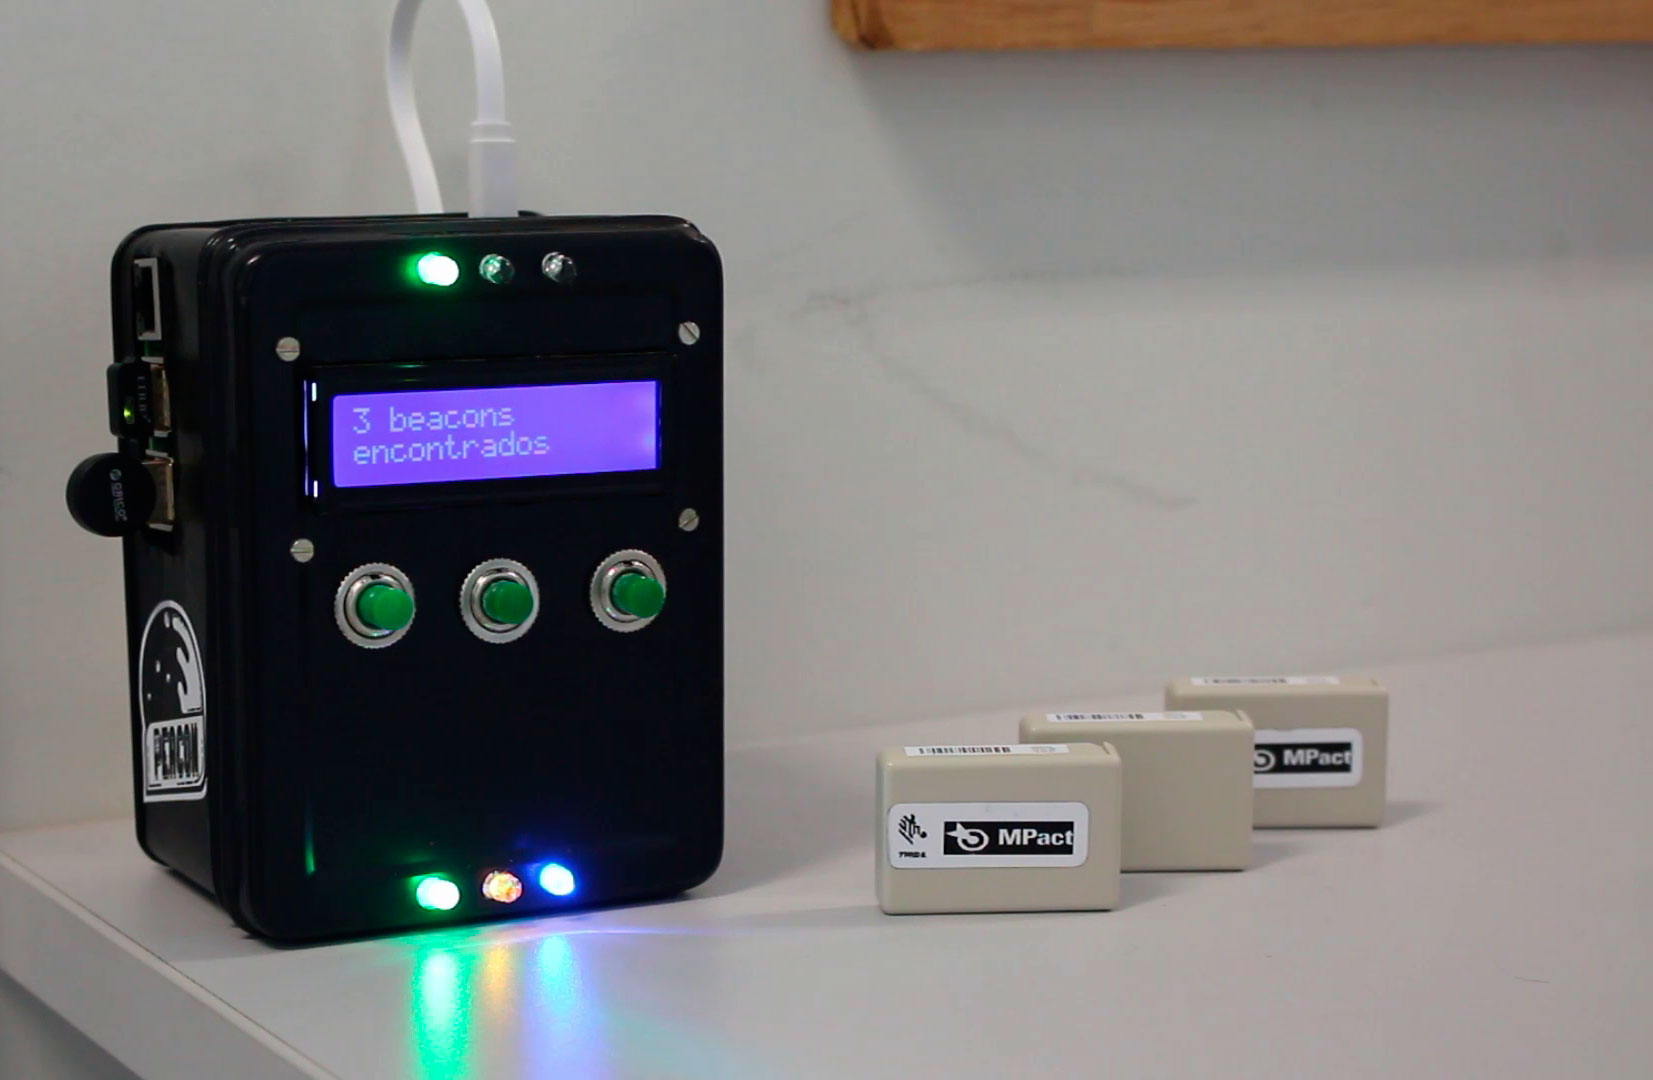
\includegraphics[width=1\textwidth]{img/peacon2.jpg}
		\legend{Fonte: elaborado pelo autor}
	\end{minipage}
\end{figure}

\begin{figure}[htb]
	\centering
 	\begin{minipage}{0.45\textwidth}
		\centering
		\caption{\label{fig:peacon3}Identificação do smartphone}
		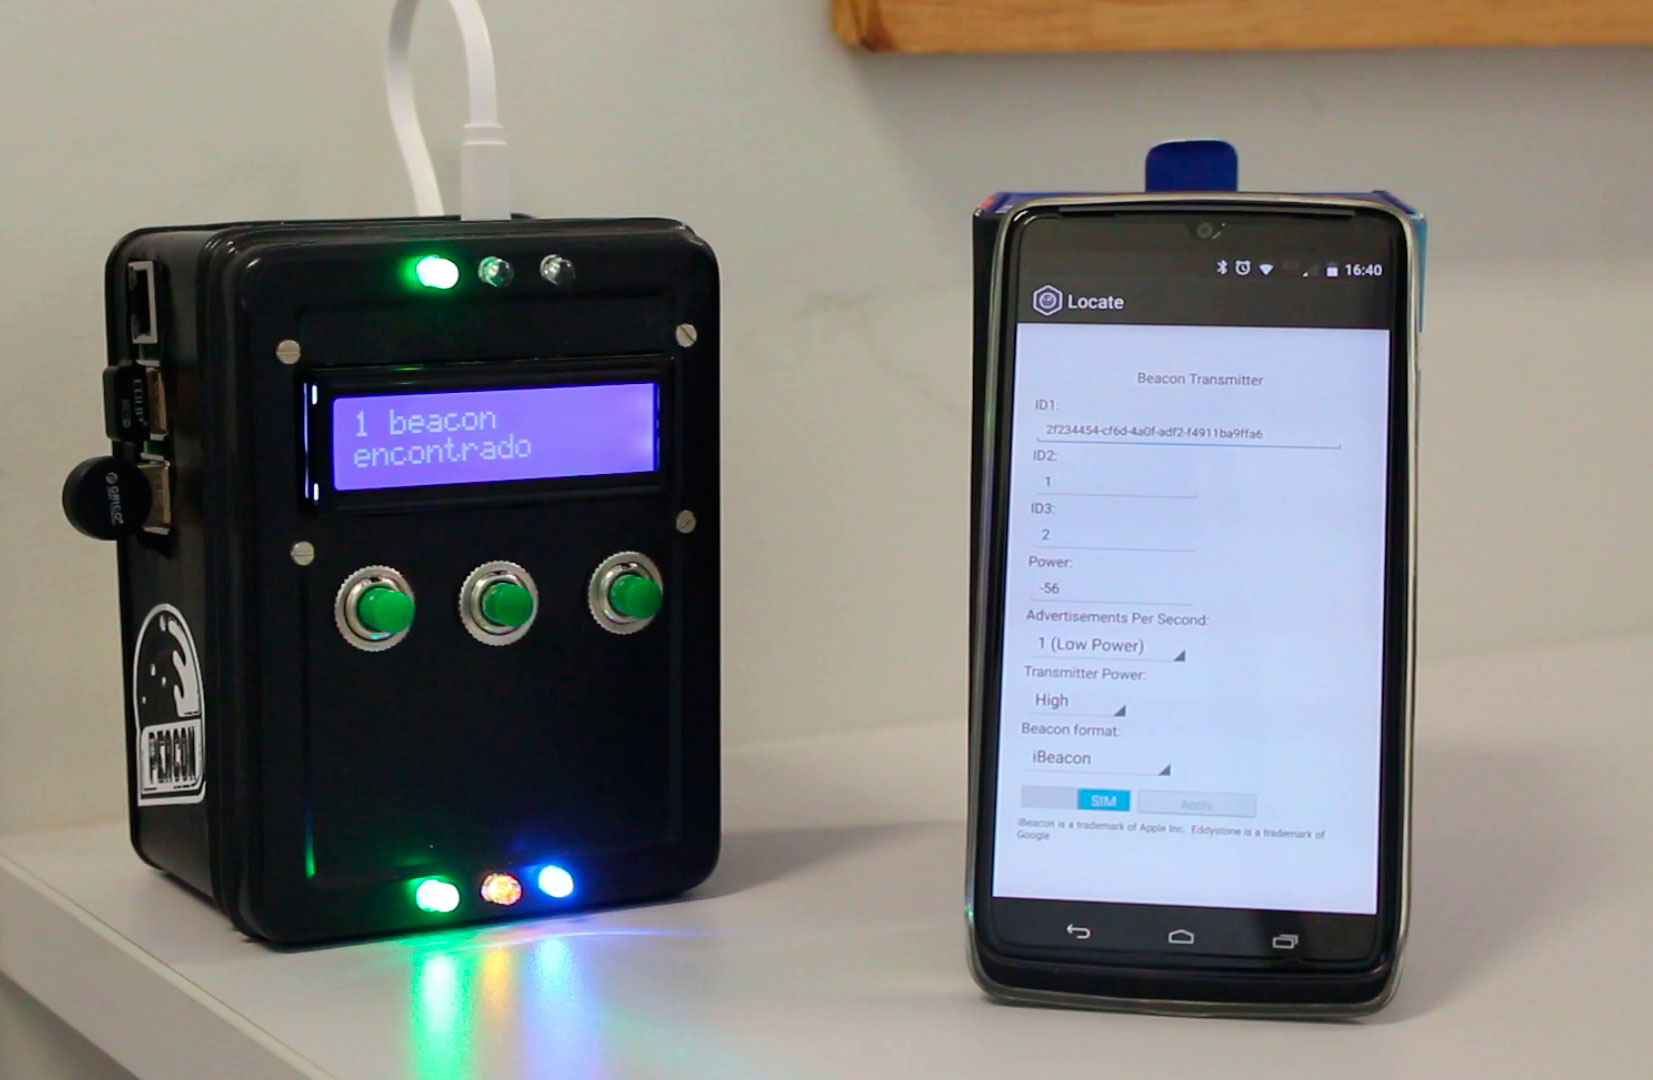
\includegraphics[width=1\textwidth]{img/peacon3.jpg}
		\legend{Fonte: elaborado pelo autor}
	\end{minipage}
	\hfill
	\begin{minipage}{0.45\textwidth}
		\centering
		\caption{\label{fig:peacon4}Identificação do smartphone e \textit{beacon}}
		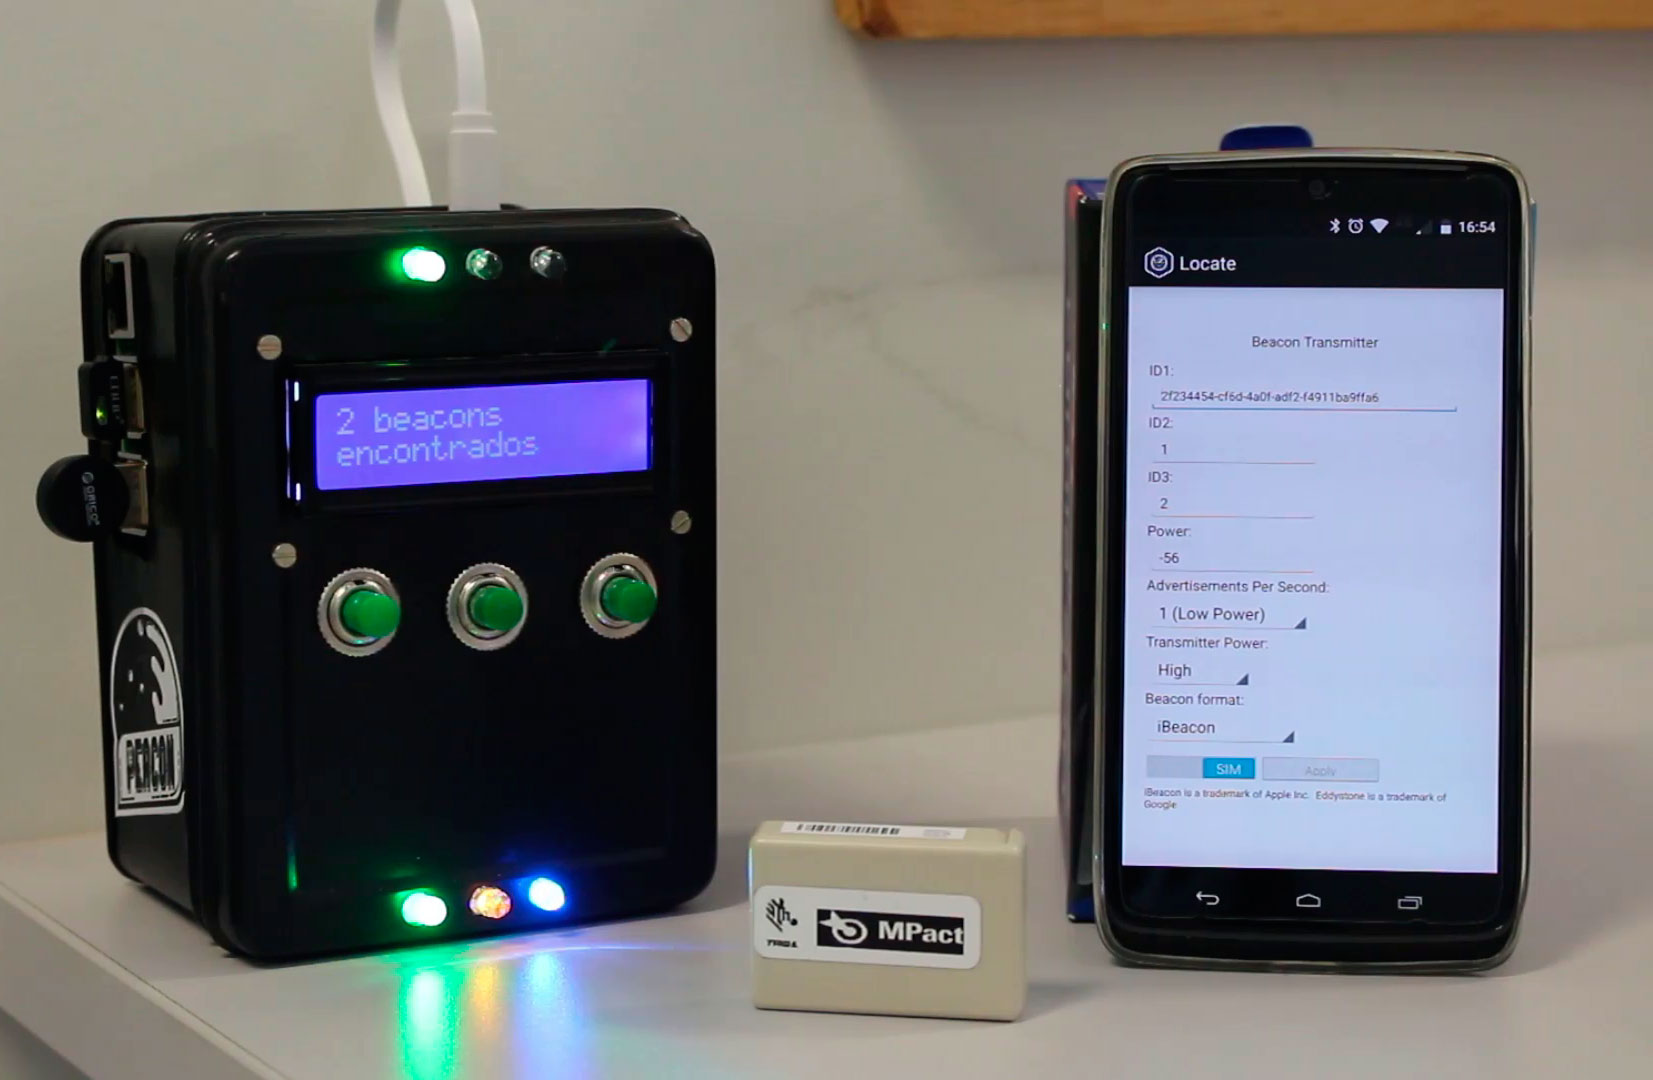
\includegraphics[width=1\textwidth]{img/peacon4.jpg}
		\legend{Fonte: elaborado pelo autor}
	\end{minipage}
\end{figure}

Todos os testes foram repetidos durante diferentes momentos do dia, durante duas semanas. Os resultados foram:

\begin{alineas}
	\item misturar os dispositivos (\textit{beacon} MPact e smartphones/tablets) não afetou em nenhum ponto - a recepção de todos continuavam normalmente, sem interferência;
	\item o protótipo suportou quatro \textit{beacons} no alcance, simultaneamente, sendo três MPact e o Moto Maxx transmitindo pacotes;
	\item \textit{beacons} em movimento apresentaram pouca ou nenhuma recepção - quando parados, apresentavam recepção constante e também um maior alcance;
	\item quando no bolso da calça, o alcance ficou extremamente limitado - inclusive parado, a distância até o protótipo era muito pouca, no máximo 30cm. Isso se deve pelo \textit{beacon} ser de baixa potência.
\end{alineas}

% ----------------------------------------------------------
\section{Avaliação do Peacon}\label{sec:prototipo-final}
% ----------------------------------------------------------

O Peacon foi desenvolvido com sucesso (\autoref{fig:prod-final}), todos os parâmetros foram satisfeitos e os testes e resultados apresentaram uma boa implementação do código. Melhorias para futuros protótipos podem ser elencadas:

\begin{alineas}
	\item Baterias internas para facilitar a execução em ambientes sem tomada próxima;
	\item Utilizar LEDs mais fracos ou resistores mais fortes;
	\item Utilizar um melhor adaptador \textit{bluetooth}, de preferência com antenas removíveis para adaptação das antenas dentro do protótipo;
	\item Colocar o \textit{RPi} totalmente dentro da caixa, deixando somente as portas necessárias.
\end{alineas}

Interessante notar que todas essas melhorias não são cruciais, mas para uma evolução e maior praticidade do produto final.

\begin{figure}[htb]
	\caption{\label{fig:prod-final}Protótipo finalizado e totalmente funcional}
	\begin{center}
		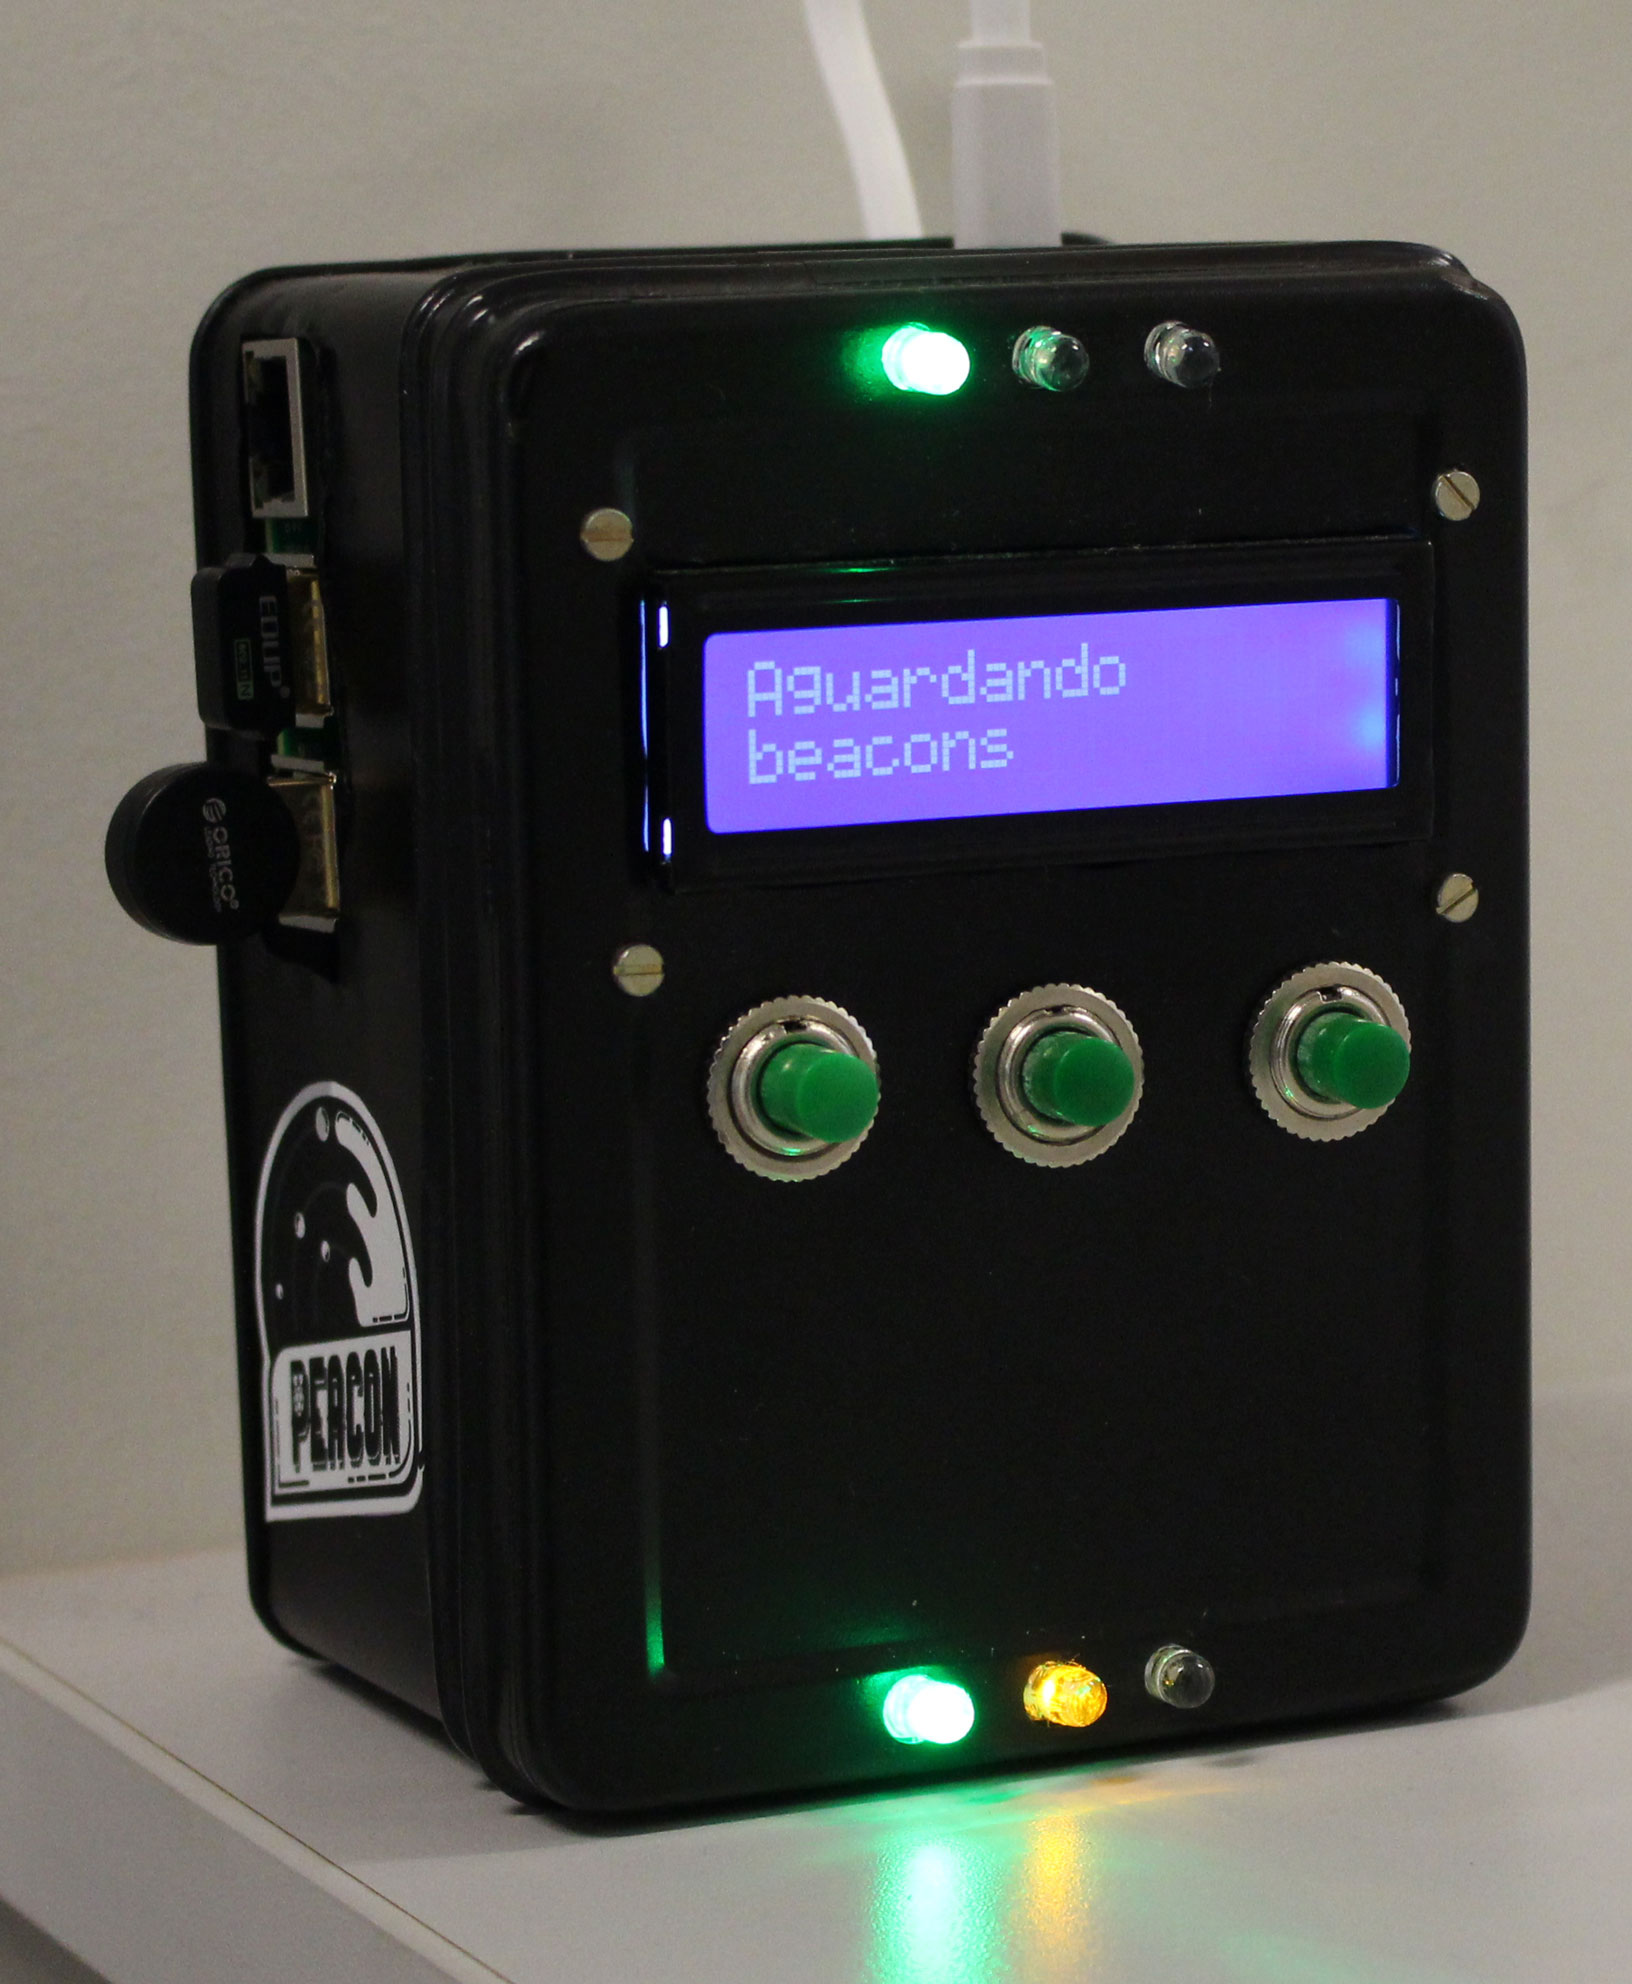
\includegraphics[width=0.65\textwidth]{img/prod-final.jpg}
	\end{center}
	\legend{Fonte: elaborado pelo autor}
\end{figure}

% ----------------------------------------------------------
